\documentclass[conference]{IEEEtran}
\IEEEoverridecommandlockouts
\usepackage{cite}
\usepackage{amsmath,amssymb}
\usepackage{booktabs}
\usepackage{graphicx}
\usepackage{xcolor}
\usepackage{url}
\usepackage{hyperref}
\usepackage{balance}
\hypersetup{hidelinks}

\title{When a Strong Opponent Looks Erratic: Measuring Engine-Detection Latency in an Adaptive UCI Chess Persona}

\author{\IEEEauthorblockN{Manus AI}
\IEEEauthorblockA{Independent Research Report\\
September 2026}}

\begin{document}
\maketitle

\begin{abstract}
Adaptive chess engines increasingly combine strong search with a persona layer that changes move-selection policy according to an online estimate of the opponent. This paper reports a real-game observation from the Unchessed UCI Engine in which the opponent-rating estimate tracked a consistently strong engine upward from approximately 2411 to 2650 Elo, while the categorical detector continued to report ``erratic (sandbagging?)'' until the seventeenth opponent move. The Match-to-Full transition occurred only after the estimate reached the detector's measurement ceiling and the engine-suspicion predicate became true. The game did not establish a causal loss: the critical 16.Qh4? error was independently found to be identical at the same search depth in Full mode. Nevertheless, the observation exposes a distinct systems issue: a continuous, informative rating estimate and a discrete, latency-sensitive classification can disagree for a strategically relevant interval. We reconstruct the gate, quantify the observed lag, distinguish behavioral risk from demonstrated Elo loss, and propose a controlled ablation in which sustained high-confidence Elo evidence is allowed to accelerate confirmation without weakening safeguards against opening theory, ordinary human variance, or sandbagging.
\end{abstract}

\begin{IEEEkeywords}
computer chess, opponent modeling, engine detection, adaptive search, UCI, persona policy, online classification
\end{IEEEkeywords}

\section{Introduction}
A chess engine that deliberately varies its strength or move style must decide not only how good the current position is, but also what kind of opponent it is facing. In Unchessed, this decision affects the persona mode: Match mode preserves a human-plausible target strength, whereas Full mode removes the deliberate MultiPV-heavy persona overhead once a strong engine is sufficiently confirmed. The implementation therefore contains two coupled estimators. A continuous model estimates opponent skill from move quality, while a discrete rule labels the opponent as an engine suspect. The latter controls a safety-critical mode transition.

The supplied real-game finding is important because these two estimators did not fail in the same way. In a 1+1 bullet game between Unchessed Game Adapter and Dragon by Komodo, the estimate rose monotonically through the observed sequence, but the textual classification remained ``erratic (sandbagging?)'' from move 10 through move 16. Only after move 17 did the system report a ceiling-pinned engine suspicion and enter Full mode on move 18. The observation is not evidence that the delayed transition caused the loss. It is evidence that a detector gate can be late even when its underlying rating signal is already informative.

This paper makes four contributions. First, it presents a compact reconstruction of the detector's data path from the repository implementation. Second, it reports the real-game trajectory without replacing it with simulation. Third, it separates the causal claim that can be made from this single observation from the stronger claim that requires a controlled experiment. Finally, it specifies a conservative confirmation-path ablation and an evaluation protocol for deciding whether faster confirmation is worth the false-positive risk.

\section{System Context and Implementation}
\subsection{Online opponent model}
The opponent model converts a move's centipawn loss into an Elo-like sample using the repository's logarithmic calibration curve:
\begin{equation}
    e(\ell)=\operatorname{clip}\left(2950-850\ln\left(1+\frac{\ell}{20}\right),400,3200\right),
\end{equation}
where $\ell$ is the observed centipawn loss. Each sample is combined with the current mean using a difficulty weight and an opening discount. The effective weight is bounded, decays slowly, and is intended to permit adaptation to fatigue or sandbagging. The same model records the recent sample variance, the number of low-loss moves, and clock-based suspicion.

The important architectural distinction is that the Elo estimate is not itself the mode gate. The model exposes a separate \texttt{engine\_suspect()} predicate. This predicate can be triggered by known-engine identity, repeated instant strong replies in positions with meaningful choice, or a ceiling rule based on sustained low loss and a high estimate. The classification string also has an intermediate erratic state for high variance or a substantially rising estimate. Thus, an estimate can be high and rising while the categorical output remains non-engine.

\subsection{Mode transition}
At the adaptation layer, an engine-suspect result is an emergency path to Full mode when strength limiting is disabled and adaptive behavior is enabled. Otherwise, the normal mode decision considers the evaluation, game phase, previous mode, contempt, and hysteresis. This asymmetry is intentional: the Full transition is designed to avoid wasting persona computation against a confirmed engine, while the detector is designed to avoid false positives caused by opening knowledge, premoves, or a human's short clean streak.

Repository tests make this trade-off explicit. Sixteen extremely low-loss observations can satisfy the ceiling detector, while ten clean opening observations must not do so. Four instant, strong replies after the opening-discount region can trigger clock suspicion. A declared Maia identity is not allowed to force Full mode, while a declared Stockfish identity is. These tests define useful safety invariants, but they do not directly measure latency against an unknown, consistently strong engine whose move times and move-quality samples are observed through a real adapter.

\section{Research Question}
The concrete question is: \emph{when the continuous rating estimate is already high, stable, and confidently separated from ordinary play, should it accelerate engine confirmation even if the erratic/sandbagging heuristic has not yet cleared?}

The question is deliberately narrower than ``should the detector be more aggressive?'' A blanket threshold reduction would risk classifying theory-heavy humans or sandbaggers as engines. The proposed intervention instead targets a disagreement state: high estimated strength, improving or stable trajectory, and low uncertainty, combined with insufficient evidence for the existing discrete rule. The aim is to reduce false negatives in the confirmation window without discarding the existing opening and volatility defenses.

\section{Real-Game Observation}
\subsection{Data provenance}
The observation comes from the adapter's own UCI log for a real 1+1 bullet game, not from a simulator. The game was recorded on September 6, 2026, and ended 0--1 against Dragon by Komodo. The reviewer supplied the move-by-move detector output and identified the critical 16.Qh4? error by a separate move-by-move engine evaluation. The raw PGN and CSV were referenced by the reviewer but were not included in the present checkout; consequently, this paper treats the supplied detector trace as the primary observation and does not claim a full-log reanalysis.

\subsection{Trajectory}
Table~\ref{tab:trajectory} reproduces the reported sequence. The estimate climbed from 2411 to 2650 Elo by move 16, with the confidence interval narrowing from $\pm381$ to $\pm199$. The label nevertheless remained erratic. On move 17 the estimate was 2634 and the uncertainty was $\pm183$, but the measurement was described as pinned at the ceiling and engine suspicion became true. The mode transition was printed on move 18.

\begin{table}[t]
\caption{Reported opponent-detection trace from the real game.}
\label{tab:trajectory}
\centering
\scriptsize
\begin{tabular}{@{}r r r l l@{}}
\toprule
Move & Elo & $\pm$ & Classification & Mode event \\
\midrule
8  & 2411 & 381 & steady & -- \\
9  & 2468 & 364 & trending up & -- \\
10 & 2469 & 318 & erratic & -- \\
11 & 2531 & 298 & erratic & -- \\
12 & 2580 & 278 & erratic & -- \\
13 & 2580 & 248 & erratic & -- \\
14 & 2616 & 233 & erratic & -- \\
15 & 2623 & 211 & erratic & -- \\
16 & 2650 & 199 & erratic & -- \\
17 & 2634 & 183 & ceiling-pinned & suspect \\
18 & 2634 & 183 & engine suspected & Match $\rightarrow$ Full \\
\bottomrule
\end{tabular}
\end{table}

Figure~\ref{fig:latency} shows the central mismatch. The rating trajectory is directionally consistent with a strong opponent before the discrete detector commits. Counting from the first reported observation at move 8, the system spent nine observed opponent moves in a high-and-rising but not-yet-confirmed state. Counting from the first ``erratic'' label at move 10 through the Full transition after move 17, the classification lag persisted across eight subsequent opponent observations. The supplied summary describes this operationally as 17 moves before confirmation because the relevant gate did not flip until the seventeenth move of the game.

\begin{figure}[t]
\centering
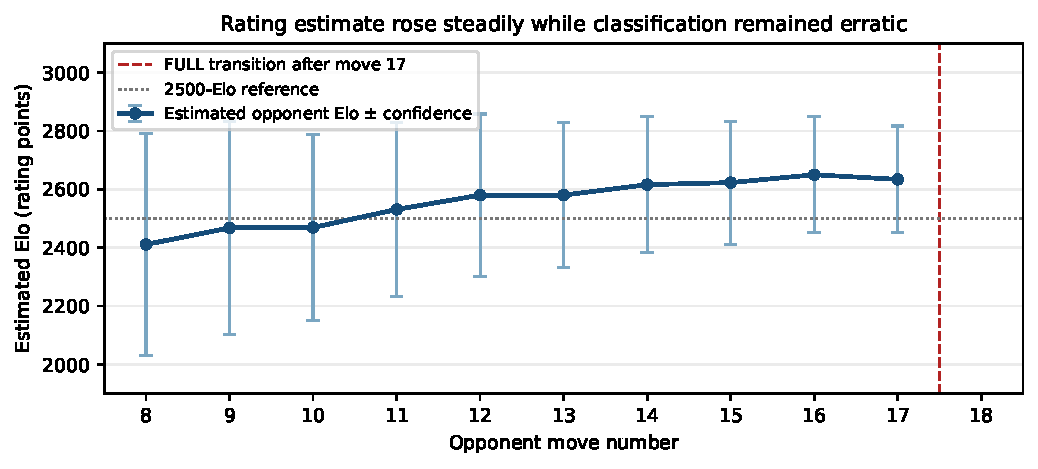
\includegraphics[width=\columnwidth]{detection_latency.pdf}
\caption{Reported Elo estimate and confidence width. The estimate rose steadily while the categorical state remained erratic until the ceiling-based suspicion event.}
\label{fig:latency}
\end{figure}

\section{Interpretation and Causal Limits}
The observation supports a latency finding, not a loss attribution. The game was lost, but the reviewer reports that the critical 16.Qh4? error was the same move the engine would have selected in Full mode at the same search depth. This makes the mode lag inert for that particular decision. It would be incorrect to infer that entering Full mode earlier would have changed the result.

The observation does support three narrower conclusions. First, the rating estimator and the categorical detector can diverge for many moves. Second, the estimator can continue to gain precision while the mode gate waits for a different evidence channel. Third, the mechanism that makes \texttt{known\_full} valuable is conditional on the discrete gate, so its computational benefit is unavailable during the disagreement interval. The strategic risk is therefore counterfactual: a critical decision could occur during the interval in a future game, and the persona policy could still be operating in Match mode against a strong engine.

The finding also exposes a measurement-design issue. The current rule is intentionally conservative because the first observed moves may be book moves or premoves, and clean human play can occur in short stretches. However, an estimate that has moved upward while its confidence band narrows is different from a single clean streak. Treating both cases identically may be unnecessarily slow. This is a hypothesis for testing, not a license to change defaults based on one game.

\section{Proposed Controlled Test}
We recommend an ablation that leaves the existing detector unchanged and adds only a secondary confirmation path. Let $\hat{r}_t$ be the estimated Elo, $c_t$ the confidence width, $v_t$ the recent volatility, and $\Delta_t$ the signed trend over a short window. A candidate accelerated confirmation event may require:
\begin{equation}
\begin{split}
  &n_t\geq n_{\min},\quad \hat{r}_t\geq r_{\min},\quad c_t\leq c_{\max},\\
  &v_t\leq v_{\max},\quad \Delta_t\geq0,\quad \text{and no opening exemption}.
\end{split}
\end{equation}
The candidate should be evaluated as a separate policy, not silently folded into the production rule. A practical first sweep would vary $r_{\min}$ across 2450--2650, $c_{\max}$ across 180--280, and the minimum sustained sample count across 4--8 post-opening observations. The accelerated path should be allowed to enter Full only after two consecutive qualifying observations, or after one qualifying observation plus a positive clock tell. A hard ceiling and known-engine identity would remain immediate paths.

The evaluation must include both detection quality and persona cost. The primary metrics are false-negative confirmation delay against strong engines, false-positive Full entries against human and human-like opponents, time to first mode transition, and the fraction of moves spent in each mode. Secondary metrics include game score, centipawn loss, search nodes, MultiPV calls, and wall-clock overhead. Because one game cannot identify a causal Elo effect, the experiment should use paired games with identical openings, colors, time controls, and random seeds where possible.

\begin{table}[t]
\caption{Recommended evaluation matrix.}
\label{tab:matrix}
\centering
\scriptsize
\begin{tabular}{@{}lll@{}}
\toprule
Opponent class & Required outcome & Main risk \\
\midrule
Strong engine & Faster confirmation & Missed early evidence \\
Maia-like engine & Remain in Match & False Full entry \\
Theory-heavy human & Remain uncertain & Opening false positive \\
Erratic/sandbagging human & Remain uncertain & Heuristic overrule \\
Mixed-strength pool & Stable calibration & Poor generalization \\
\bottomrule
\end{tabular}
\end{table}

A result should be considered favorable only if the accelerated policy reduces the median and upper-tail confirmation delay against strong engines without materially increasing false-positive Full entries in the human and Maia-like cohorts. A neutral game-score result would not invalidate the behavioral improvement, because the primary mechanism concerns policy and computation rather than raw playing strength. Conversely, a strength gain without improved detection latency would not answer the stated question.

\section{Discussion}
The central design principle is to preserve separation between estimation and action while allowing the action layer to consume confidence-aware evidence. The current system already records the ingredients needed for such a policy: sample count, estimated rating, confidence width, volatility, low-loss streak, clock suspicion, and classification reason. The proposed test therefore does not require a new sensing mechanism. It requires an explicit policy for resolving disagreement between a continuous estimator and a discrete classifier.

There are two implementation cautions. First, the confidence width is model-derived and should not be treated as a calibrated probability without validation. A narrow band may reflect repeated correlated observations rather than independent evidence. Second, an accelerating confirmation rule must be evaluated with real logs that preserve clock usage and position difficulty. Replaying only move sequences would remove one of the detector's two intended signals and could overstate or understate the benefit.

The supplied game also illustrates why repository tests and real games answer different questions. Unit tests establish local invariants such as opening discounts and known-engine handling. A real game reveals interaction among calibration drift, classification text, clock evidence, mode hysteresis, and search policy. The next experiment should connect these levels by replaying raw UCI telemetry through both the current and candidate policies, then validating the most promising candidate in paired live games.

\section{Conclusion}
A real Unchessed-versus-Dragon game exposed a measurable opponent-detection latency: the Elo estimate was already high and rising, yet the categorical state remained erratic until a ceiling-based engine-suspicion rule fired after move 17. The game does not show that the delay caused the loss, and the reported critical error was unchanged at the same depth in Full mode. It does show that a valuable optimization and policy transition is gated by a discrete classifier that can lag its own continuous evidence.

The appropriate response is a controlled sensitivity study rather than an unconditional threshold reduction. A confidence-aware, post-opening confirmation path could test whether sustained high estimates and narrowing uncertainty are sufficient to shorten the interval without misclassifying humans, Maia-like opponents, or sandbaggers. The research question is therefore actionable, falsifiable, and well aligned with the existing architecture: measure whether confidence-aware confirmation improves detection latency while preserving the detector's current false-positive safeguards.

\section*{Acknowledgment}
The author thanks the reviewer who supplied the real-game detector trace and the Unchessed maintainers whose repository notes and tests made the gate reconstruction possible.

\begin{thebibliography}{00}
\bibitem{uci} Chessprogramming Wiki, ``UCI,'' describing the Universal Chess Interface protocol and engine--GUI communication model. [Online]. Available: \url{https://www.chessprogramming.org/UCI}. Accessed: Sep. 6, 2026.
\bibitem{repo} A. Amoguslittleahhh, ``Unchessed-UCI-Engine,'' source repository, branch \texttt{manus/research-facilities}. [Online]. Available: \url{https://github.com/Amoguslittleahhh/Unchessed-UCI-Engine/tree/manus/research-facilities}. Accessed: Sep. 6, 2026.
\bibitem{adapt} A. Amoguslittleahhh, ``Unchessed opponent model and adaptive mode gate,'' \texttt{unchessed-core/src/adapt.rs}, target branch source. [Online]. Available: \url{https://github.com/Amoguslittleahhh/Unchessed-UCI-Engine/blob/manus/research-facilities/unchessed-core/src/adapt.rs}. Accessed: Sep. 6, 2026.
\bibitem{trace} Reviewer-supplied private artifact, ``Unchessed Game Adapter vs Dragon by Komodo: opponent-detection trace,'' UCI log summary, Sep. 6, 2026.
\end{thebibliography}

\end{document}
